\chapter{Revisão Sistemática da Literatura}
\label{cap:rsl}

A Revisão Sistemática da Literatura (RSL) constituiu a primeira etapa da pesquisa e teve como objetivo consolidar evidências empíricas sobre estratégias de \textit{design}, técnicas arquiteturais, métricas de avaliação e lacunas relacionadas a sistemas intensivos em dados. Essa etapa fornece a base conceitual e empírica para a campanha experimental e para a proposta de um modelo de apoio à decisão arquitetural.

A RSL resultou no artigo intitulado \textit{Design of Data-Intensive Systems: A Systematic Review with Exploratory Quantitative Synthesis}, submetido ao WEBIST 2026. No momento da elaboração desta proposta, o artigo encontra-se aguardando aprovação. Essa submissão representa um dos resultados parciais desta pesquisa e consolida a etapa de revisão sistemática desenvolvida no âmbito da dissertação.

A condução da revisão seguiu diretrizes reconhecidas para Revisões Sistemáticas da Literatura em Engenharia de Software \cite{kitchenham2007guidelines,kitchtchenham2009,kitchenham2015evidence} e utilizou o protocolo PRISMA 2020 como referência para relatar o processo de identificação, triagem, elegibilidade e inclusão dos estudos \cite{page2021prisma}. Além da síntese qualitativa, foi conduzida uma síntese quantitativa exploratória com o objetivo de comparar, de forma normalizada, os efeitos de diferentes otimizações arquiteturais reportadas na literatura.

\section{Objetivo e Questões de Pesquisa}
\label{sec:rsl-objetivo}

O objetivo da RSL foi identificar, organizar e sintetizar evidências sobre o \textit{design} de sistemas intensivos em dados, com ênfase em estratégias arquiteturais orientadas ao desempenho. A revisão buscou responder às seguintes questões de pesquisa:

\begin{enumerate}
    \item Quais técnicas e abordagens de \textit{design} são aplicadas em sistemas intensivos em dados?
    \item Quais métricas são utilizadas para avaliar o desempenho e a eficiência desses sistemas?
    \item Quais evidências quantitativas existem sobre a efetividade das diferentes abordagens?
    \item Quais estilos arquiteturais, \textit{frameworks} ou padrões de \textit{design} são mais recorrentes em sistemas intensivos em dados?
    \item Existem lacunas ou oportunidades para estudos futuros?
\end{enumerate}

Essas questões permitiram orientar a busca, a seleção, a extração dos dados e a análise dos estudos primários. A definição das questões também contribuiu para delimitar o foco da revisão, evitando a inclusão de estudos genéricos sobre \textit{Big Data} que não apresentassem relação direta com \textit{design} arquitetural, métricas de desempenho ou avaliação empírica.

\section{Estratégia de Busca}
\label{sec:rsl-estrategia-busca}

A busca foi realizada em quatro bibliotecas digitais: ACM Digital Library\footnote{\url{https://dl.acm.org/}}, IEEE Xplore\footnote{\url{https://ieeexplore.ieee.org}}, Scopus\footnote{\url{https://www.scopus.com}} e ScienceDirect\footnote{\url{https://www.sciencedirect.com/}}. Essas bases foram selecionadas por sua relevância para as áreas de Engenharia de Software, Sistemas Distribuídos, Arquitetura de Software e Computação Intensiva em Dados.

A estratégia de busca foi construída com base na estrutura PICO, considerando quatro dimensões principais: população, intervenção, comparação e resultado (\textit{outcome}). A população foi representada por termos associados a sistemas intensivos em dados, como \textit{data-intensive systems}, \textit{big data systems} e \textit{large-scale data systems}. A intervenção foi representada por termos relacionados a \textit{design}, arquitetura e projeto arquitetural. A comparação incluiu termos associados a atributos de qualidade, como desempenho, escalabilidade, confiabilidade e tolerância a falhas. O resultado foi representado por termos relacionados a métricas e avaliação quantitativa.

De forma geral, a \textit{string} de busca combinou os termos por meio de operadores booleanos, conforme a lógica apresentada a seguir:

\begin{equation}
S = (P) \land (I) \land (C) \land (O)
\label{eq:string-pico}
\end{equation}

em que $P$ representa os termos associados à população, $I$ representa os termos associados à intervenção, $C$ representa os termos associados aos atributos comparativos e $O$ representa os termos associados aos resultados esperados. Essa formulação permitiu estruturar a busca de modo sistemático e alinhado ao objetivo da revisão.

A busca foi conduzida em setembro de 2025. Foram considerados estudos publicados em periódicos revisados por pares ou em anais de conferências, desde que apresentassem relação direta com sistemas intensivos em dados, \textit{design} arquitetural, avaliação de desempenho ou otimizações sistêmicas.

\section{Critérios de Inclusão e Exclusão}
\label{sec:rsl-criterios}

Para assegurar a relevância e a qualidade dos estudos selecionados, foram definidos critérios de inclusão e exclusão antes da execução da triagem. Esses critérios foram aplicados nas etapas de leitura de títulos, resumos e textos completos.

\begin{table}[htbp]
\centering
\caption{Critérios de inclusão e exclusão da RSL}
\label{tab:criterios-rsl}
\footnotesize
\setlength{\tabcolsep}{6pt}
\renewcommand{\arraystretch}{1.3}
\begin{tabular}{p{6.2cm} p{6.2cm}}
\toprule
\textbf{Critérios de Inclusão} & \textbf{Critérios de Exclusão} \\ 
\midrule
Estudos publicados em periódicos revisados por pares ou conferências. & Estudos puramente conceituais, sem resultados empíricos. \\ 
Estudos sobre \textit{design}, arquitetura ou implementação de sistemas intensivos em dados. & Trabalhos sem métricas quantitativas ou sem descrição do ambiente experimental. \\ 
Trabalhos que comparam a solução proposta com pelo menos uma configuração de referência (\textit{baseline}). & Estudos não escritos em inglês. \\ 
Pesquisas com resultados quantitativos, como desempenho, escalabilidade ou consumo de recursos. & Trabalhos sobre sistemas de dados em geral, sem foco específico em sistemas intensivos em dados ou \textit{design} arquitetural. \\ 
Estudos com texto completo disponível e documentação mínima do ambiente experimental. & Revisões de literatura, meta-análises, cartas, editoriais ou capítulos de livro. \\ 
\bottomrule
\multicolumn{2}{l}{\footnotesize Fonte: elaborado pelo autor.}
\end{tabular}
\end{table}

Nos casos em que houve dúvidas sobre a aplicação dos critérios, a decisão foi discutida entre os revisores. Quando não foi possível alcançar consenso, um avaliador independente foi consultado. As razões de exclusão foram registradas ao longo do processo, garantindo maior transparência e rastreabilidade à revisão.

\section{Processo de Seleção dos Estudos}
\label{sec:rsl-selecao}

O processo de busca nas quatro bibliotecas digitais identificou 979 registros. A distribuição inicial foi de 448 artigos na ACM Digital Library, 215 na IEEE Xplore, 35 na ScienceDirect e 281 na Scopus. Após a remoção de 100 duplicatas, restaram 879 estudos únicos para a etapa de triagem.

A triagem por títulos e resumos resultou na exclusão de 600 registros que não atendiam aos critérios estabelecidos. Em seguida, 279 textos completos foram avaliados. Nessa etapa, 269 estudos foram excluídos, principalmente por não apresentarem resultados quantitativos compatíveis com o foco da síntese, por não descreverem adequadamente o ambiente experimental ou por não permitirem comparação com uma configuração de referência.

Ao final do processo, 10 estudos atenderam a todos os critérios de elegibilidade e qualidade, sendo incluídos tanto na Revisão Sistemática da Literatura quanto na síntese quantitativa exploratória.

A Figura~\ref{fig:prisma-rsl} apresenta o fluxo de seleção dos estudos de acordo com o modelo PRISMA 2020.

\begin{figure}[htbp]
\centering
\begin{tikzpicture}[
node distance=0.7cm,
caixa/.style={
rectangle,
draw,
align=center,
text width=5.2cm,
minimum height=0.9cm,
font=\small
},
seta/.style={-{Latex[length=3mm]}, thick}
]
\node[caixa] (id) {Registros identificados \\ $n = 979$};
\node[caixa, below=of id] (dup) {Duplicatas removidas \\ $n = 100$};
\node[caixa, below=of dup] (triados) {Registros triados \\ $n = 879$};
\node[caixa, right=1.5cm of triados] (excluidos) {Registros excluídos \\ $n = 600$};
\node[caixa, below=of triados] (full) {Textos completos avaliados \\ $n = 279$};
\node[caixa, right=1.5cm of full] (fullex) {Textos completos excluídos \\ $n = 269$};
\node[caixa, below=of full] (incluidos) {Estudos incluídos na RSL \\ $n = 10$};
\node[caixa, below=of incluidos] (sintese) {Estudos na síntese quantitativa \\ $n = 10$};

\draw[seta] (id) -- (dup);
\draw[seta] (dup) -- (triados);
\draw[seta] (triados) -- (full);
\draw[seta] (full) -- (incluidos);
\draw[seta] (incluidos) -- (sintese);
\draw[seta] (triados) -- (excluidos);
\draw[seta] (full) -- (fullex);
\end{tikzpicture}
\caption{Fluxo PRISMA 2020 do processo de seleção dos estudos}
\label{fig:prisma-rsl}
\end{figure}

A Tabela~\ref{tab:distribuicao-bases} apresenta a distribuição dos registros identificados por base de dados.

\begin{table}[htbp]
\centering
\caption{Distribuição dos registros identificados por base de dados}
\label{tab:distribuicao-bases}
\small
\begin{tabular}{p{6cm} p{4cm}}
\toprule
\textbf{Base de dados} & \textbf{Registros identificados} \\ 
\midrule
ACM Digital Library & 448 \\ 
IEEE Xplore & 215 \\ 
ScienceDirect & 35 \\ 
Scopus & 281 \\ 
\midrule
\textbf{Total} & \textbf{979} \\ 
\bottomrule
\multicolumn{2}{l}{\footnotesize Fonte: elaborado pelo autor.}
\end{tabular}
\end{table}

\section{Avaliação da Qualidade}
\label{sec:rsl-qualidade}

A avaliação da qualidade dos estudos foi conduzida com base em um \textit{checklist} composto por 14 critérios. Esses critérios avaliaram aspectos como clareza do problema, aderência ao tema, descrição do contexto, metodologia, uso de dados experimentais, métricas arquiteturais, replicabilidade, limitações, recomendações práticas, apresentação de valores numéricos, comparabilidade das métricas, descrição do ambiente experimental, medidas de dispersão e comparação entre técnicas ou arquiteturas.

Cada critério recebeu uma das seguintes pontuações: Sim = 1, Parcialmente = 0,5 e Não = 0. Considerando os 14 critérios, a pontuação máxima possível para cada estudo foi de 14 pontos. Foi adotado um ponto de corte de 8 pontos, correspondente a aproximadamente 60\% da pontuação máxima, conforme representado pela Equação~\ref{eq:qa-score}.

\begin{equation}
QA_{min} = 0.60 \times 14 = 8.4 \approx 8
\label{eq:qa-score}
\end{equation}

Apenas estudos que atingiram ou superaram esse limiar foram mantidos no conjunto final. A adoção desse critério buscou garantir que os estudos incluídos apresentassem qualidade metodológica mínima para sustentar a síntese qualitativa e a síntese quantitativa exploratória.

\begin{table}[htbp]
\centering
\caption{Dimensões avaliadas no checklist de qualidade}
\label{tab:dimensoes-qualidade}
\small
\setlength{\tabcolsep}{6pt}
\renewcommand{\arraystretch}{1.3}
\begin{tabular}{p{4cm} p{8cm}}
\toprule
\textbf{Dimensão} & \textbf{Aspectos avaliados} \\ 
\midrule
Clareza do estudo & Definição do problema, objetivo e aderência ao \textit{design} de sistemas intensivos em dados. \\ 
Contexto experimental & Descrição do sistema, volume de dados, ambiente de execução, \textit{hardware}, \textit{software} e \textit{workload}. \\ 
Métricas e resultados & Uso de métricas quantitativas, apresentação de valores numéricos e comparabilidade dos resultados. \\ 
Rigor metodológico & Metodologia clara, replicabilidade, uso de \textit{baseline} e apresentação de limitações. \\ 
Relevância prática & Diretrizes, recomendações ou implicações para o \textit{design} de sistemas intensivos em dados. \\ 
\bottomrule
\multicolumn{2}{l}{\footnotesize Fonte: elaborado pelo autor.}
\end{tabular}
\end{table}

\section{Extração dos Dados}
\label{sec:rsl-extracao}

Os dados foram extraídos por meio de um formulário padronizado, implementado em uma planilha previamente definida. Para cada estudo incluído, foram registrados os seguintes campos: identificação do estudo, autores, ano de publicação, veículo de publicação, base digital, tipo de sistema investigado, domínio de aplicação, técnica arquitetural ou otimização proposta, métricas utilizadas e resultados quantitativos reportados.

Também foram extraídas informações relacionadas ao ambiente experimental, incluindo \textit{hardware}, \textit{software}, \textit{datasets}, \textit{workloads}, número de execuções, médias, desvios-padrão, variâncias e demais medidas estatísticas, quando disponíveis. A extração foi conduzida por um revisor principal e verificada por um segundo revisor. Divergências foram resolvidas por discussão e, quando necessário, por consulta a um terceiro avaliador.

Essa etapa foi essencial para permitir tanto a síntese qualitativa quanto a síntese quantitativa exploratória, uma vez que os estudos selecionados apresentavam métricas heterogêneas e diferentes formas de relato experimental.

\section{Síntese Quantitativa Exploratória}
\label{sec:rsl-sintese-quantitativa}

Em vez de realizar uma meta-análise inferencial formal, esta pesquisa adotou uma síntese quantitativa exploratória. Essa decisão foi motivada pela ausência sistemática de medidas de variância, desvio-padrão e tamanho amostral em grande parte dos estudos primários. Diante dessa limitação, a ponderação individual dos estudos e a modelagem formal de efeitos aleatórios não seriam estatisticamente defensáveis.

Para permitir comparações entre estudos que utilizaram métricas heterogêneas, foi adotada a Razão de Resposta Logarítmica, ou \textit{Log Response Ratio} (LRR), como medida normalizada de efeito. De forma geral, o LRR pode ser definido como:

\begin{equation}
LRR_i = \ln(RR_i)
\label{eq:lrr}
\end{equation}

em que $RR_i$ representa a razão de resposta do estudo $i$. Quando a métrica analisada indicava que valores maiores eram melhores, como \textit{throughput} ou \textit{speedup}, a razão foi calculada conforme a Equação~\ref{eq:rr-maior-melhor}.

\begin{equation}
RR_i = \frac{M_{tratamento}}{M_{baseline}}
\label{eq:rr-maior-melhor}
\end{equation}

Quando a métrica indicava que valores menores eram melhores, como tempo de execução, latência ou tempo de recuperação, a razão foi invertida, conforme a Equação~\ref{eq:rr-menor-melhor}.

\begin{equation}
RR_i = \frac{M_{baseline}}{M_{tratamento}}
\label{eq:rr-menor-melhor}
\end{equation}

A média não ponderada dos valores de LRR foi utilizada para estimar a magnitude geral dos efeitos observados:

\begin{equation}
\overline{LRR} = \frac{1}{k}\sum_{i=1}^{k} LRR_i
\label{eq:lrr-medio}
\end{equation}

em que $k$ representa o número de estudos incluídos na síntese quantitativa. Para facilitar a interpretação, o LRR médio também pode ser convertido novamente para a escala de razão de resposta:

\begin{equation}
RR_{medio} = e^{\overline{LRR}}
\label{eq:rr-medio}
\end{equation}

Como o valor médio observado foi $\overline{LRR} = 0.981$, a razão média de resposta foi aproximadamente:

\begin{equation}
RR_{medio} = e^{0.981} \approx 2.7
\label{eq:rr-resultado}
\end{equation}

Esse resultado indica que, de forma exploratória, as otimizações analisadas apresentaram impacto médio positivo no desempenho, com ganhos aproximados de $2,7$ vezes em relação às configurações de referência. No entanto, esse valor deve ser interpretado com cautela, pois a síntese não utiliza ponderação por variância ou tamanho amostral.

\section{Estudos Incluídos e Resultados}
\label{sec:rsl-estudos-incluidos}

Os dez estudos incluídos na síntese quantitativa exploratória investigam diferentes tipos de otimizações em sistemas intensivos em dados, abrangendo desde técnicas de escalonamento e compilação SQL até estratégias de armazenamento, processamento próximo aos dados e tolerância a falhas \cite{wang2018hard,aung2019coordinate,alquwaiee2022performance,ponce2019upgrading,li2022karst,vincon2020nkv,lyu2022fine,haynes2016pipegen,schiavio2020dynamic,gotze2018nvm-aware}.

A Tabela~\ref{tab:estudos-lrr} apresenta uma síntese dos estudos incluídos, suas otimizações principais, métricas utilizadas e valores de LRR.

\begin{table}[htbp]
\centering
\caption{Síntese dos estudos primários incluídos na RSL}
\label{tab:estudos-lrr}
\textfloatsep=10pt
\footnotesize
\setlength{\tabcolsep}{4pt}
\renewcommand{\arraystretch}{1.25}
\begin{tabular}{p{3.2cm} p{4.2cm} p{3.2cm} r}
\toprule
\textbf{Estudo} & \textbf{Otimização principal} & \textbf{Métrica analisada} & \textbf{LRR} \\ 
\midrule
Wang et al. (2018) & Escalonamento em Spark/YARN & Taxa de conclusão & 0,233 \\ 
Aung et al. (2019) & Tolerância a falhas com \textit{checkpoint} & Tempo de recuperação & 0,357 \\ 
AlQuwaiee et al. (2022) & Modelagem de desempenho em Spark & Tempo de execução & 0,511 \\ 
Ponce et al. (2019) & Integração entre HPC e \textit{Big Data} & \textit{Throughput} & 0,631 \\ 
Li et al. (2022) & Protocolo transacional escalável & \textit{Throughput} & 0,693 \\ 
Vin{\c{c}}on et al. (2020) & Processamento próximo aos dados & Desempenho & 0,993 \\ 
Lyu et al. (2022) & Gerenciamento fino de recursos & Latência/custo & 1,273 \\ 
Haynes et al. (2016) & Geração de \textit{pipelines} de dados & \textit{Speedup} & 1,335 \\ 
Schiavio et al. (2020) & Otimização dinâmica de compilação & \textit{Speedup} & 1,482 \\ 
G{\"o}tze et al. (2018) & Layout de armazenamento para NVM & Desempenho & 2,303 \\ 
\bottomrule
\multicolumn{4}{l}{\footnotesize Fonte: elaborado pelo autor.}
\end{tabular}
\end{table}

Os resultados indicam que as maiores magnitudes de efeito estão associadas a intervenções em baixo nível, especialmente aquelas relacionadas a armazenamento, movimentação de dados e execução de consultas. Em contraste, otimizações em camadas de controle, como escalonamento e tolerância a falhas, apresentaram ganhos mais moderados, embora ainda relevantes do ponto de vista arquitetural.

\section{Distribuição Temática dos Estudos}
\label{sec:rsl-distribuicao-tematica}

A análise dos estudos incluídos permitiu agrupá-los em três categorias temáticas principais: otimização de consultas e execução, otimização de hardware e armazenamento, e integração e conectividade. A primeira categoria correspondeu a 40\% dos estudos, enquanto as duas demais representaram 30\% cada.

A Figura~\ref{fig:distribuicao-tematica} apresenta a distribuição temática dos estudos incluídos.

\begin{figure}[htbp]
\centering
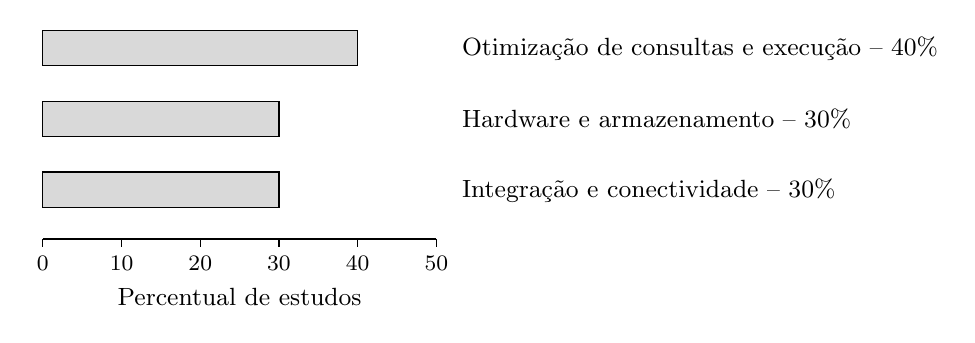
\begin{tikzpicture}

\draw[fill=gray!30] (0,1.4) rectangle (4,1.85);
\draw[fill=gray!30] (0,0.5) rectangle (3,0.95);
\draw[fill=gray!30] (0,-0.4) rectangle (3,0.05);


\node[anchor=west] at (5.2,1.62) {\small Otimização de consultas e execução -- 40\%};
\node[anchor=west] at (5.2,0.72) {\small Hardware e armazenamento -- 30\%};
\node[anchor=west] at (5.2,-0.18) {\small Integração e conectividade -- 30\%};


\draw[thick] (0,-0.8) -- (5,-0.8);

\foreach \x/\label in {0/0, 1/10, 2/20, 3/30, 4/40, 5/50} {
    \draw (\x,-0.8) -- (\x,-0.9);
    \node[anchor=north] at (\x,-0.9) {\footnotesize \label};
}
\node[anchor=north] at (2.5,-1.3) {\small Percentual de estudos};
\end{tikzpicture}
\caption{Distribuição temática dos estudos incluídos}
\label{fig:distribuicao-tematica}
\end{figure}

A categoria de otimização de consultas e execução inclui estudos relacionados ao escalonamento, à compilação SQL e ao gerenciamento de recursos. A categoria de hardware e armazenamento concentra estudos sobre memória não volátil, processamento próximo aos dados e protocolos transacionais escaláveis. A categoria de integração e conectividade reúne estudos voltados à eficiência na movimentação de dados, integração entre ambientes e tolerância a falhas.

Essa distribuição evidencia que parte significativa das contribuições da literatura está concentrada em camadas de execução e infraestrutura. Esse resultado reforça a importância de decisões arquiteturais que considerem não apenas a organização lógica do sistema, mas também aspectos de baixo nível, como armazenamento, movimentação de dados, execução de consultas e gerenciamento de recursos.

\section{Lacunas Identificadas}
\label{sec:rsl-lacunas}

A RSL permitiu identificar lacunas importantes na literatura sobre \textit{design} de sistemas intensivos em dados. A primeira lacuna refere-se à ausência de padronização no relato experimental. Muitos estudos reportam métricas como tempo de execução, latência, \textit{throughput} e \textit{speedup}, mas nem sempre apresentam informações suficientes sobre o número de execuções, medidas de dispersão, intervalos de confiança ou detalhes completos do ambiente experimental. Essa limitação dificulta a replicação dos estudos e restringe a realização de meta-análises inferenciais.

A segunda lacuna está relacionada à heterogeneidade das métricas e dos cenários avaliados. Embora os estudos investiguem sistemas intensivos em dados, as técnicas, \textit{workloads}, \textit{datasets}, ambientes e métricas variam significativamente. Essa diversidade reforça a necessidade de medidas normalizadas, como o LRR, mas também exige cautela na interpretação dos resultados agregados.

A terceira lacuna refere-se à concentração dos estudos em otimizações específicas. Muitos trabalhos analisam técnicas pontuais em ambientes controlados, mas poucos oferecem diretrizes gerais para apoiar decisões arquiteturais em contextos variados. Como consequência, ainda há necessidade de abordagens que auxiliem arquitetos de software a relacionar características dos dados, estratégias de processamento e métricas de desempenho.

A quarta lacuna envolve a limitada integração entre características dos dados e decisões arquiteturais. A maioria dos estudos avalia o desempenho a partir de métricas operacionais, mas poucos investigam como propriedades dos dados, como distribuição, cardinalidade, redundância, variabilidade ou entropia, podem influenciar a escolha entre alternativas arquiteturais. Essa lacuna sustenta a proposta desta dissertação de investigar uma abordagem quantitativa de apoio à decisão arquitetural baseada em evidências empíricas e características observáveis dos dados.

A partir dessas lacunas, a RSL fornece a base metodológica e empírica para as próximas etapas da pesquisa. Seus resultados justificam a condução da campanha experimental apresentada no Capítulo~\ref{cap:campanha-experimental} e fundamentam a proposta de um modelo quantitativo de apoio à decisão arquitetural em sistemas intensivos em dados.
